\chapter{Cycles énergétiques}
\section{Cycle du soleil}

\section{Cycle circadien humain}
% cycles d’environ 24 heures
% Synchronisation par la lumiere du jour au niveaux de l’hypothamus
% le niveau de mélatonine sanguin est très faible le jour
% Plus la lumière diminue d’intensité, plus ce niveau augmente pour atteindre un degré maximal de sécrétion entre deux et quatre heures du matin

% Le cycle est different en fonction de l'age
% Newborn babies: They still don’t have a well formed circadian cycle, that’s the reason why they sleep on and off. As their sleep cycle gets more consolidated, daytime naps are less frequent and sleep is consolidated during the night.
% Children: Children need more sleep than adults, 11-13 hours per night between age 3-5 and 10-11 hours between 6 and 9 years old.
% Teenagers: Hormonal shifts change the circadian rhythm, making them go to bed later at night, and waking them up later in the morning.
% Adults: Adults needs between 7-9 hours of sleep every night. Some lifestyle choices, such as consumption of caffeine, stress and screen use during the evening disrupt our sleep cycle.


% Activitees pouvant de-regler le cycle :
% - Blue LED lightning, commonly emitted by screens, reduces melatonin production. This impacts our ability to fall asleep. We strongly encourage you to use blue light filters during the evening .
% - Travail de nuit

% Sources
% https://fondationsommeil.com/le-cycle-circadien/
% https://en.getmoona.com/blogs/mission-sleep/how-your-circadian-rhythm-influences-your-sleep

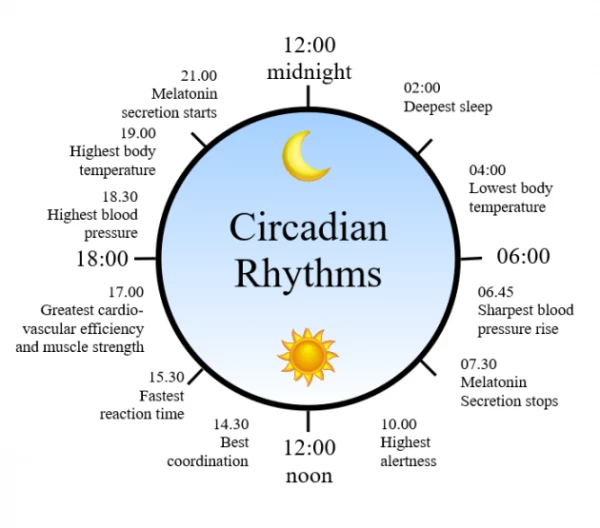
\includegraphics[scale=1.00]{media/circadien.png}

\section{Cycles long cours}
% Cette partie parlera des differents cycles terrestres prenant cours sur le long terme
% ex. Courants marins - Point chaud
\section{Équilibre de la production}

\section{Anticipation de la consommation}
